\documentclass[12pt]{article}
\input{../../preamble.tex}
\newcommand{\F}{\mathcal{F}}
\newcommand{\f}[2]{\mathcal{F}\{#1\}(\omega) = \int_{-\infty}^{\infty}#2e^{-2\pi i\omega t}dt}
\newcommand{\finverse}[2]{\mathcal{F}^{-1}\{#1\}(t) = \int_{-\infty}^{\infty}#2e^{2\pi i\omega t}d\omega}
\usepackage{listings}
\usepackage[margin=1.0in]{geometry}
\usepackage{setspace}
\DeclareMathOperator{\spn}{span}
\title{Fourier Analysis}
\doublespacing
\begin{document}
    \maketitle
    \tableofcontents

    \section{Fourier Analysis}
    Fourier Analysis is the study of functions in their relation to the Fourier Transform: \[\hat{f}(\omega) = \f{f}{f(t)}\] And the Inverse Fourier Transform: \[f(t) = \finverse{\hat{f}}{\hat{f}(\omega)}\]
    These operators transform a function between it's time domain ($f(t)$) and it's frequency domain ($\hat{f}(\omega)$), which can be used to decompose a function into a series of trigonometric functions that approximate the function. This allows for functions, sets, or even images, to be expressed in a much simpler format. Due to this fact, Fourier Analysis is incredibly useful in the world of image and audio compression and decompression, and can even be used to filter out certain frequencies from audio and certain colors from images.
    \section{Fourier Series}
    An \emph{integral} part of calculus and linear algebra deals with approximating functions and representing them as polynomials, which is known as a Taylor Series. The $n$th degree taylor polynomial for some function $f(x)$ is defined by a polynomial  $p_n(x) \in \spn\{1, x, x^2,\ldots,x^n\}$ that closely approximates $f(x)$. The function $p_n(x)$ centered at $x=b$ takes the form of a series  \[ p_n(x)=\sum_{k=0}^n \frac{f^{(k)}(b)(x-b)^k}{k!}\] Where $f^{(k)}(b)$ denotes the  $k$th derivative of  $f$ at  $b$. Taking the limit  \[\lim_{n \to \infty} p_n(x) = \lim_{n \to \infty} \sum_{k=0}^n \frac{f^{(k)}(b)(x-b)^k}{k!} = f(x)\] So any infinitely differentiable function can be represented by this series.\\\\
    The taylor series of a function is, in a way, the most basic form of functional series of a function; it is a vector in the polynomial space, however it can be shown that any function $f(x)$ can be represented as a sum of any even and odd functions, which makes sense when we examine the basis $\{1, x, x^2,\ldots,x^n\}$ and rearrange it as $\{1,x^2,x^4,\ldots,x^n,x,x^3,x^5,\ldots,x^{n-1}\}$, assuming $n$ is even \cite{directsums}. Using this, it might make sense to study a new type of series that is formed by a different basis of even and odd functions, which is where the Fourier Series comes into play. As trigonometric functions have many applications in math, physics, and the natural sciences, it would make sense that a series that uses them as a basis also has many applications. This series is known as the \textbf{\emph{Fourier Series}}, which brings us to Fourier's Theorem: 
    \begin{theorem}[Fourier's Theorem]
        Any (reasonably well-behaved)\footnote{Fourier Series converge for periodic functions which are "nice:" ones which have first and second derivatives which, along with the function itself, have a finite number of dscontinuities and zero crossings on the interval of their period \cite{reed}} function can be written in terms of trigonometric or exponential functions \cite{harvard}.
    \end{theorem}
    This follows from the idea that two orthogonal functions (ones with an inner product $\langle f, g \rangle = \int f(x)g(x)dx = 0$) can form an orthogonal basis for the function space $\mathbb{F}$ \cite{linalg}. It can be shown that  $f(t) = \sin(nt)$ and $g(t) = \cos(mt)$ are orthogonal as follows:
    \begin{align}
        \langle \sin(nt), \cos(mt) \rangle = & \int_{0}^{2\pi}\sin(nt)\cos(mt)dt \\
                           = & \int_{0}^{2\pi} \frac{1}{2}[\sin(nt+mt)+\sin(nt-mt)dt \\
                           = & 0
    \end{align}
    \note{We can introduce bounds on the integral because both $\sin$ and $\cos$ are $2\pi$-periodic.}
    \subsection{Trigonometric Series}
    From this theorem, it follows that $\sin(nt)$ and $\cos(mt)$ form an orthogonal basis for $\mathbb{F}$, that is, $\spn{\{1, \cos(t), \cos(2t),\ldots,\cos(mt),\sin(t),\sin(2t),\ldots,\sin(nt)\}} = \mathbb{F}$. This proves Fourier's Theorem, which means any function can be expressed as
    \begin{align}
        f(x) = & \sum_{n=0}^{\infty} \left[ a_n\cos\left(\frac{2\pi n x}{L}\right) + b_n\sin\left( \frac{2\pi n x}{L} \right)\right] \\
        = & \frac{a_0}{2} + \sum_{n=1}^{\infty} \left[ a_n\cos\left(\frac{2\pi n x}{L}\right) + b_n\sin\left( \frac{2\pi n x}{L} \right)\right]
    \end{align}
    Where $a_n$ and $b_n$ are some coefficients (which we will derive shortly) and  $L$ is the period of the function  $f(x)$. To find the coefficients, we must start with the initial representation of the function:
    \begin{align}
        f(x) &= \sum_{n=0}^{\infty}\left[ a_n\cos\left(\frac{2\pi n x }{L}\right) + b_n\sin\left( \frac{2\pi n x}{L} \right)  \right] \\
        \int_0^L f(x) \cos\left( \frac{2\pi m x}{L} \right)dx &= \int_0^L \sum_{n=0}^{\infty} \left[ a_n\cos\left(\frac{2\pi n x}{L}\right) + b_n\sin\left( \frac{2\pi n x}{L} \right)\right] \cos\left(\frac{2\pi m x}{L}\right)dx \\
                                      &= \sum_{n=0}^{\infty} \left[ \int_0^L a_n\cos\left(\frac{2\pi n x}{L}\right)\cos\left(\frac{2\pi m x}{L}\right) + b_n\sin\left( \frac{2\pi n x}{L} \right)\cos\left(\frac{2\pi m x}{L}\right)dx \right] \\
                                      &= \sum_{n=0}^{\infty} \left[ \int_0^L a_n\cos\left(\frac{2\pi n x}{L}\right)\cos\left(\frac{2\pi m x}{L}\right)dx \right] \\
                                      &= \sum_{n=0}^{\infty} \left[ \frac{a_n}{2}\int_0^L \cos\left((m-n)\frac{2\pi x}{L}\right)dx \right] \\ 
                                      &= \frac{a_mL}{2} \\
                                      &\implies a_n = \frac{2}{L}\int_0^L f(x)\cos\left( \frac{2\pi n x}{L} \right)dx
    \end{align}
    Which means
    \begin{align}
        a_0 = & \frac{2}{L}\int_0^Lf(x)\cos\left( 0\cdot\frac{2\pi x}{L} \right)dx \\
        = & \frac{2}{L}\int_0^L f(x)dx
    \end{align}
    And we can employ similar reasoning to show that \[b_n = \frac{2}{L}\int_0^Lf(x)\sin\left( \frac{2\pi n x}{L} \right)dx\] And since $f(x)$ must be $L$-periodic, the bounds of the integral, the only condition is that the interval of integration is of length $L$ \cite{harvard}.
    \subsection{Exponentials}
    Fourier's Theorem also tells us that we can write functions in term of exponential functions, so it makes sense that there is a closed form for an exponential, complex Fourier Series. Starting with the definition of the Fourier Series from (4) and introducing the substitution $\omega = \frac{2\pi}{L}$ for ease of use we have
    \begin{align}
        f(x) &= \frac{a_0}{2} + \sum_{n=1}^{\infty}\left[ a_n\cos\left( \omega n x \right) + b_n\sin\left( \omega n x \right) \right] \\
             &= \frac{a_0}{2} + \sum_{n=1}^{\infty}\left[ a_n\frac{e^{i\omega n x}+e^{-i\omega n x}}{2} + b_n\frac{e^{i\omega n x}-e^{-i\omega n x}}{2i}\right] \\
             &= \frac{a_0}{2} + \sum_{n=1}^{\infty}\left[ \frac{a_n-b_ni}{2} e^{i\omega n t} \right] +\sum_{n=1}^{\infty}\left[ \frac{a_n+b_ni}{2}e^{-i\omega n t} \right] \\
        n = -n \text{ for part 2 of (17)} &\implies \frac{a_0}{2} + \sum_{n=1}^{\infty}\left[ \frac{a_n-b_ni}{2} e^{i\omega n t} \right] +\sum_{n=-1}^{-\infty}\left[ \frac{a_{-n}+b_{-n}i}{2}e^{i\omega n t} \right] \\
        \implies f(x) &= \sum_{n = -\infty}^{\infty}\left[ C_n e^{2\pi i n x / L} \right]
    \end{align}
    Where \[C_n = \frac{1}{L} \int_0^Lf(x)e^{-2\pi i n x / L} dx\] By the same logic that we used to find the coefficients of the trigonometric series \cite{reed}.
    \section{Fourier Transform}
    One caveat of the Fourier Series is that it only works with functions that are $L$-periodic. We can get around this by starting with the formula for the exponential Fourier Series and taking $\lim_{L \to \infty}$; in other words giving a nonperiodic function a period of $[-\infty,\infty]$.
    \begin{align}
        f(x) &= \sum_{n = -\infty}^{\infty}\left[ C_n e^{2\pi i n x / L} \right] \\
             &= \sum_{n = -\infty}^{\infty}\left[ \frac{1}{L}\int_{-\frac{L}{2}}^{\frac{L}{2}} f(\omega)e^{-2\pi i n \omega / L}d\omega \cdot e^{2\pi i n x / L}\right] \\
             &= \sum_{n=-\infty}^{\infty}\left[ \frac{1}{L}\int_{-\frac{L}{2}}^{\frac{L}{2}} f(\omega)e^{2\pi i n (x-\omega) / L}\right] \\
        \tau = \frac{n}{L} &\implies \sum_{\tau = -\infty}^{\infty}\left[ \int_{-\frac{L}{2}}^{\frac{L}{2}} f(\omega)e^{2\pi i \tau (x-\omega)}d\omega \right] \\
        d\tau = \frac{1}{L} &\implies \int_{-\infty}^{\infty}\int_{-\infty}^{\infty} f(\omega)e^{2\pi i \tau(x-\omega)}d\omega d\tau \\
        \implies f(x) &= \int_{-\infty}^{\infty}\left[\int_{-\infty}^{\infty} f(\omega)e^{-2\pi i \omega x}d\omega\right] e^{2\pi i \tau x}d\tau
    \end{align}
    This result gives us some interesting information: it suggests that two very similar inverse operations differ by only a negative in the exponent, so we will define these operations as the \textbf{\emph{Fourier Transform}} $\hat{f}(\omega) = \F\{f\}$ and \textbf{\emph{Inverse Fourier Transform}} $f(t) = \F^{-1}\{\hat{f}\}$:
    \begin{align}
        \hat{f}(\omega) &= \f{f}{f(t)} \\
        f(t) &= \finverse{\hat{f}}{\hat{f}(\omega)}
    \end{align}
    And using the corresponding definition of the Fourier Series, we can see that $\hat{f}(\omega)$ is "equivalent" to the coefficients from the Series. When talking about the transform, it is often said that the Fourier Transform takes a function from the time domain to the frequency domain, meaning that while $f(t)$ contains information relating the time  $t$ to the function's value,  $\hat{f}(\omega)$ contains information relating the frequency $\omega$  to information containing both the magnitude and phase of a trigonometric function.
    \subsection{Discrete Fourier Transform}
    As was just mentioned, the Fourier Transform $\hat{f}(\omega)$ of a function encodes its fourier coefficients, so there must be a way to use this function to create a fourier series for $f(t)$. This is where we can use the \textbf{\emph{Discrete Fourier Transform}}, which is an algorithm for finding the coefficients of a function's Fourier Series at discrete intervals. This algorithm takes a discrete set of complex input points and uses the formula we developed earlier to compute the Fourier coefficients of the input function. Replacing the integral in the Fourier Transform formula we obtained earlier with a summation over all the points in some sequence of complex numbers $\{x_n\}$ with length $N$, we have
    \begin{align}
        X_k &= \sum_{n=0}^{N-1}\left[ x_n \cdot e^{-2\pi i k n / N} \right] \\
            &= \sum_{n=0}^{N-1}\left[ x_n \cdot \left( \cos\left( \frac{2\pi k n}{N} \right) - i\sin\left( \frac{2 \pi k n}{N} \right)  \right) \right]
    \end{align}
    Which can be implemented as follows:\footnote{This code was written by me which is why it does not have a citation}
    \begin{lstlisting}[language=Java, basicstyle=\small]
    HashMap<String, Double> DFT(Complex[] x) {
        HashMap<String, Double> X = new Map<String, Double>();
        int N = x.length;
        for (int k = 0; k < N; k++) {
            double re = 0; double im = 0;
            for (int n = 0; n < N; n++) {
                double angle = (2 * Math.PI * k * n) / N;
                re += x[n].re * Math.cos(angle) + x[n].im * Math.sin(angle);
                im += x[n].im * Math.cos(angle) - x[n].re * Math.sin(angle);
            }
            X.put("re", re);
            X.put("im",im);
            X.put("frequency", k);
            X.put("amplitude", Math.sqrt(re * re + im * im);
            X.put("phase", Math.atan2(im, re));
        }
    }
    \end{lstlisting}
    This algorithm has $O(n^2)$, however a more efficient algorithm can be implemented when $N$ is a power of  $2$.
    \subsubsection{The FFT}
    The Fast Fourier Transform, or FFT, is an algorithm for computing a function's Discrete Fourier Transform quickly and efficiently. It only works when the input sequence is of a power of $2$ length, however it admits  $O(n\log n)$, which greatly makes up for it in efficiency. The FFT can be implemented as follows \cite{fft}:
    \begin{lstlisting}[language=Java, basicstyle=\small]
    Complex[] fft(Complex[] x) {
        int n = x.length;

        // base case
        if (n == 1) return new Complex[] { x[0] };

        // radix 2 Cooley-Tukey FFT
        if (n % 2 != 0) {
            throw new IllegalArgumentException("n is not a power of 2");
        }

        // compute FFT of even terms
        Complex[] even = new Complex[n/2];
        for (int k = 0; k < n/2; k++) {
            even[k] = x[2*k];
        }
        Complex[] evenFFT = fft(even);

        // compute FFT of odd terms
        Complex[] odd  = even;  // reuse the array (to avoid n log n space)
        for (int k = 0; k < n/2; k++) {
            odd[k] = x[2*k + 1];
        }
        Complex[] oddFFT = fft(odd);

        // combine
        Complex[] y = new Complex[n];
        for (int k = 0; k < n/2; k++) {
            double kth = -2 * k * Math.PI / n;
            Complex wk = new Complex(Math.cos(kth), Math.sin(kth));
            y[k]       = evenFFT[k].plus (wk.times(oddFFT[k]));
            y[k + n/2] = evenFFT[k].minus(wk.times(oddFFT[k]));
        }
        return y;
    } 
    \end{lstlisting}
    \section{Properties of the Fourier Transform and It's Inverse}
    The Fourier Transform and it's inverse are operators, just like addition, subtraction, multiplication, and division, so it would make sense for them to have various interesting properties, which it does. Assuming $f(t)$ is a real-valued function:
    \begin{align}
        & \hat{f}(\omega) = \overline{\hat{f}(-\omega)} \\
        & \F\{f(-t)\} = \hat{f}(-\omega) \\
        & \F\left\{ \frac{d^nf(t)}{dt^n} \right\} = (-2\pi i \omega)^n\hat{f}(\omega) \\
        \intertext{And for any $f(t)$ and $g(t)$ with Fourier Transforms  $\hat{f}(\omega)$ and $\hat{g}(\omega)$}
        & \F\{af(t)\pm bg(t)\} = a\F\{f(t)\} \pm b\F\{g(t)\} \\
        & \int_{-\infty}^{\infty}\left|f(t)\right|^2dt = \int_{-\infty}^{\infty}\left|\hat{f}(\omega)\right|^2d\omega
    \end{align}
    \subsection{Convolution Theorem}
    The Convolution Theorem is kind of like a product rule for the Fourier Transform, it states that
    \begin{align}
        \F\{f(t)\cdot g(t)\} = \int_{-\infty}^{\infty} \hat{f}(\tau)\hat{g}(\omega-\tau)d\tau
    \end{align}
    Which is read "the confolution of $\hat{f}$ with $\hat{g}$, so
    \begin{align}
        \F\{f(t)\cdot g(t)\} &= \F\{f(t)\}*\F\{g(t)\} = \int_{-\infty}^{\infty}\hat{f}(\tau)\hat{g}(\omega-\tau)d\tau
    \end{align}
    And is very useful when applied to solve differential equations \cite{reed}.
    \section{Applications of Fourier Analysis}
    Several of the applications of Fourier analysis stem from physics, specifically the realm of Differential equations. Harvard Professor David Morin writes that "many (although certainly not all) of the differential equations that govern physical systems are \emph{linear}, which implies that the sum of two solutions is again a solution. Therefore, since Fourier analysis tells us that any function can be written in terms of sinusoidal functions, we can limit our attention to these function when solving the differential equations" \cite{harvard}. \\\\
    This gives us a jumping off point for many differential equations, such as the heat equation $\frac{\partial u}{\partial t} = \Delta u$, a fundamental equation in the world of physics that was Fourier's motivation to develop his particular field of analysis. \\\\
    Additionally, Fourier Series are very useful in the field of signal composition and decomposition; the Fourier Transform can be used to compress images, filter aspects of the resulting transform's frequencies, and then decompress images into either the original (if the transform was not filtered) or altered (if the transform was filtered) images.
    \begin{figure}[H]
        \centering
        \begin{subfigure}[t]{0.2\linewidth}
            \centering
            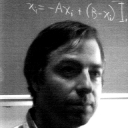
\includegraphics[width=\linewidth]{untransformed.png}
            \caption{Original Image}
        \end{subfigure}
        \begin{subfigure}[t]{0.2\linewidth}
            \centering
            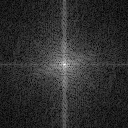
\includegraphics[width=\linewidth]{transformed.png}
            \caption{Fourier Transformed Image}
        \end{subfigure}
        \begin{subfigure}[t]{0.2\linewidth}
            \centering
            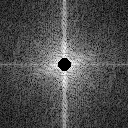
\includegraphics[width=\linewidth]{filtered-transformed.png}
            \caption{Filtered Fourier Transform}
        \end{subfigure}
        \begin{subfigure}[t]{0.2\linewidth}
            \centering
            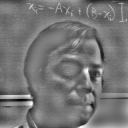
\includegraphics[width=\linewidth]{filtered-untransformed.png}
            \caption{Inverse Fourier Transformed Image}
        \end{subfigure}
        \caption{An image transformed into its Fourier Transform, filtered, and then transformed back into image form \cite{images}}
    \end{figure}
    \begin{thebibliography}{4}
        \bibitem[Ellermeyer]{directsums} Ellermeyer, S. (2008, July 21). \emph{Direct Sums of Subspaces and Fundamental Subspaces}. \url{https://ksuweb.kennesaw.edu/~sellerme/sfehtml/classes/math3260/directsumsandfundamentalsubspaces.pdf}
        \bibitem[Morin]{harvard} Morin, D. (2009). \emph{Fourier analysis.} \url{https://scholar.harvard.edu/files/david-morin/files/waves_fourier.pdf}
        \bibitem[Illing]{reed} Illing, L. (2008). \emph{FOURIER ANALYSIS}. \url{https://www.reed.edu/physics/courses/Physics331.f08/pdf/Fourier.pdf}
        \bibitem[Lehar]{images} Lehar, S. (2006, February 10). \emph{An Intuitive Explanation of Fourier Theory}. \url{Web.archive.org. https://web.archive.org/web/20060210112754/http://cns-alumni.bu.edu/~slehar/fourier/fourier.html}
    \bibitem[Lay]{linalg} Mcdonald, J., Lay, S. R., \& Lay, D. C. (2016). \emph{Linear algebra and its applications, fifth edition, David C. Lay, University of Maryland, Steven R. Lay, Lee University, Judi J. McDonald, Washington State University.} Pearson.
    \bibitem[Sedgewick]{fft} Sedgewick, R., Wayne, K. (2020, January 14). \emph{FFT.java}. Introcs.cs.princeton.edu. Retrieved May 28, 2021, from https://introcs.cs.princeton.edu/java/97data/FFT.java.html
    \end{thebibliography}
\end{document}
